この章では、FDPS Fortran/C言語 インターフェースのファイル構成と概要について記述する。はじめに
ソースファイルの構成とインターフェース概要について記述し、その後、ドキュメントとサンプルコードについて記述する。

%%%%%%%%%%%%%%%%%%%%%%%%%%%%%%%%%%%%%%%%%%%%%%%%%%%%
\section{ファイル構成と概要}
%%%%%%%%%%%%%%%%%%%%%%%%%
\subsection{FDPS 本体}
FDPS 本体のソースファイルはディレクトリ \path{src} の下にある。FDPS 本体は C++ で記述されており、FDPS の標準機能関係のソースファイルはすべて \path{src} の 直下にある。FDPS には拡張機能が用意されており、現時点では、Particle Mesh と x86 版 Phantom-GRAPE が実装されている。それぞれのソースファイルが、\path{src/particle_mesh} と \path{src/phantom_GRAPE_x86} にある。これら拡張機能は静的ライブラリとして使用される。そのため、各ディレクトリにおいて、ユーザ自身の手で、静的ライブラリを作成する必要がある。詳細はFDPS本体の仕様書(\path{doc/doc_specs_cpp_ja.pdf})をご覧頂きたい。
%%%%%%%%%%%%%%%%%%%%%%%%%
\subsection{Fortran インターフェース}
\label{subsec:file_str_ftn_if}
前節で述べた機能の内、Fortran から利用可能なのは、FDPS 標準機能(一部 API は除く)と拡張機能 Particle Mesh である。ユーザは Fortran インターフェースプログラムを通して、これらの機能を使用することとなる。この Fortran インターフェースは、ユーザがディレクトリ\path{scripts}の下に置かれたスクリプト\path{gen_ftn_if.py}を実行することで生成される(スクリプトの仕様は第\ref{chap:script_spec}章で解説する)。このインターフェース生成用スクリプトは、FDPSを利用するにあたってユーザ自身が定義(実装)しなければならない派生データ型(\textbf{ユーザ定義型};第\ref{chap:user_defined}章参照)を解析して、インターフェースプログラムを生成する。\uline{\textbf{したがって、ユーザ最初にしなければならないことはユーザ定義型の実装である}}。FDPSのFortran用のインターフェースがライブラリの形ではなく、このようなインターフェースプログラムの生成という形で提供される理由については別途第\ref{subsec:reasons_for_autogen_ftn_if}節で解説する。Fortranでユーザ定義型を実装するのに必要となるFortranファイルが\path{src/fortran_interface/modules}に、インターフェース生成時に設計図として使用されるファイル群が \path{src/fortran_interface/blueprints} に配置されている。

図\ref{fig:FDPS_ftn_if_file_str}に、Fortran用インターフェースプログラムの生成が正常に行われた場合の Fortran インターフェースのファイル構成とその役割を示している。図の破線で囲まれた4つのファイル(\path{FDPS_module.F90}, \path{FDPS_ftn_if.cpp}, \path{FDPS_Manipulators.cpp}, \path{main.cpp})がスクリプトによって生成されるFortranインターフェースプログラムであり、\path{f_main.F90}がユーザ側が用意するプログラムである。図の点線で囲まれたファイル(\path{FDPS_vector.F90}、\path{FDPS_matrix.F90}、\path{FDPS_super_particle.F90}等)は、前述したように、ユーザがユーザ定義型およびユーザ定義関数(第\ref{chap:overview}章参照)を記述するのに必要な派生データ型の定義を与える。以下、それぞれのインターフェースプログラムの役割について説明を行う。

%%% 図:全体のファイル構成
\begin{figure}[h]
\centering
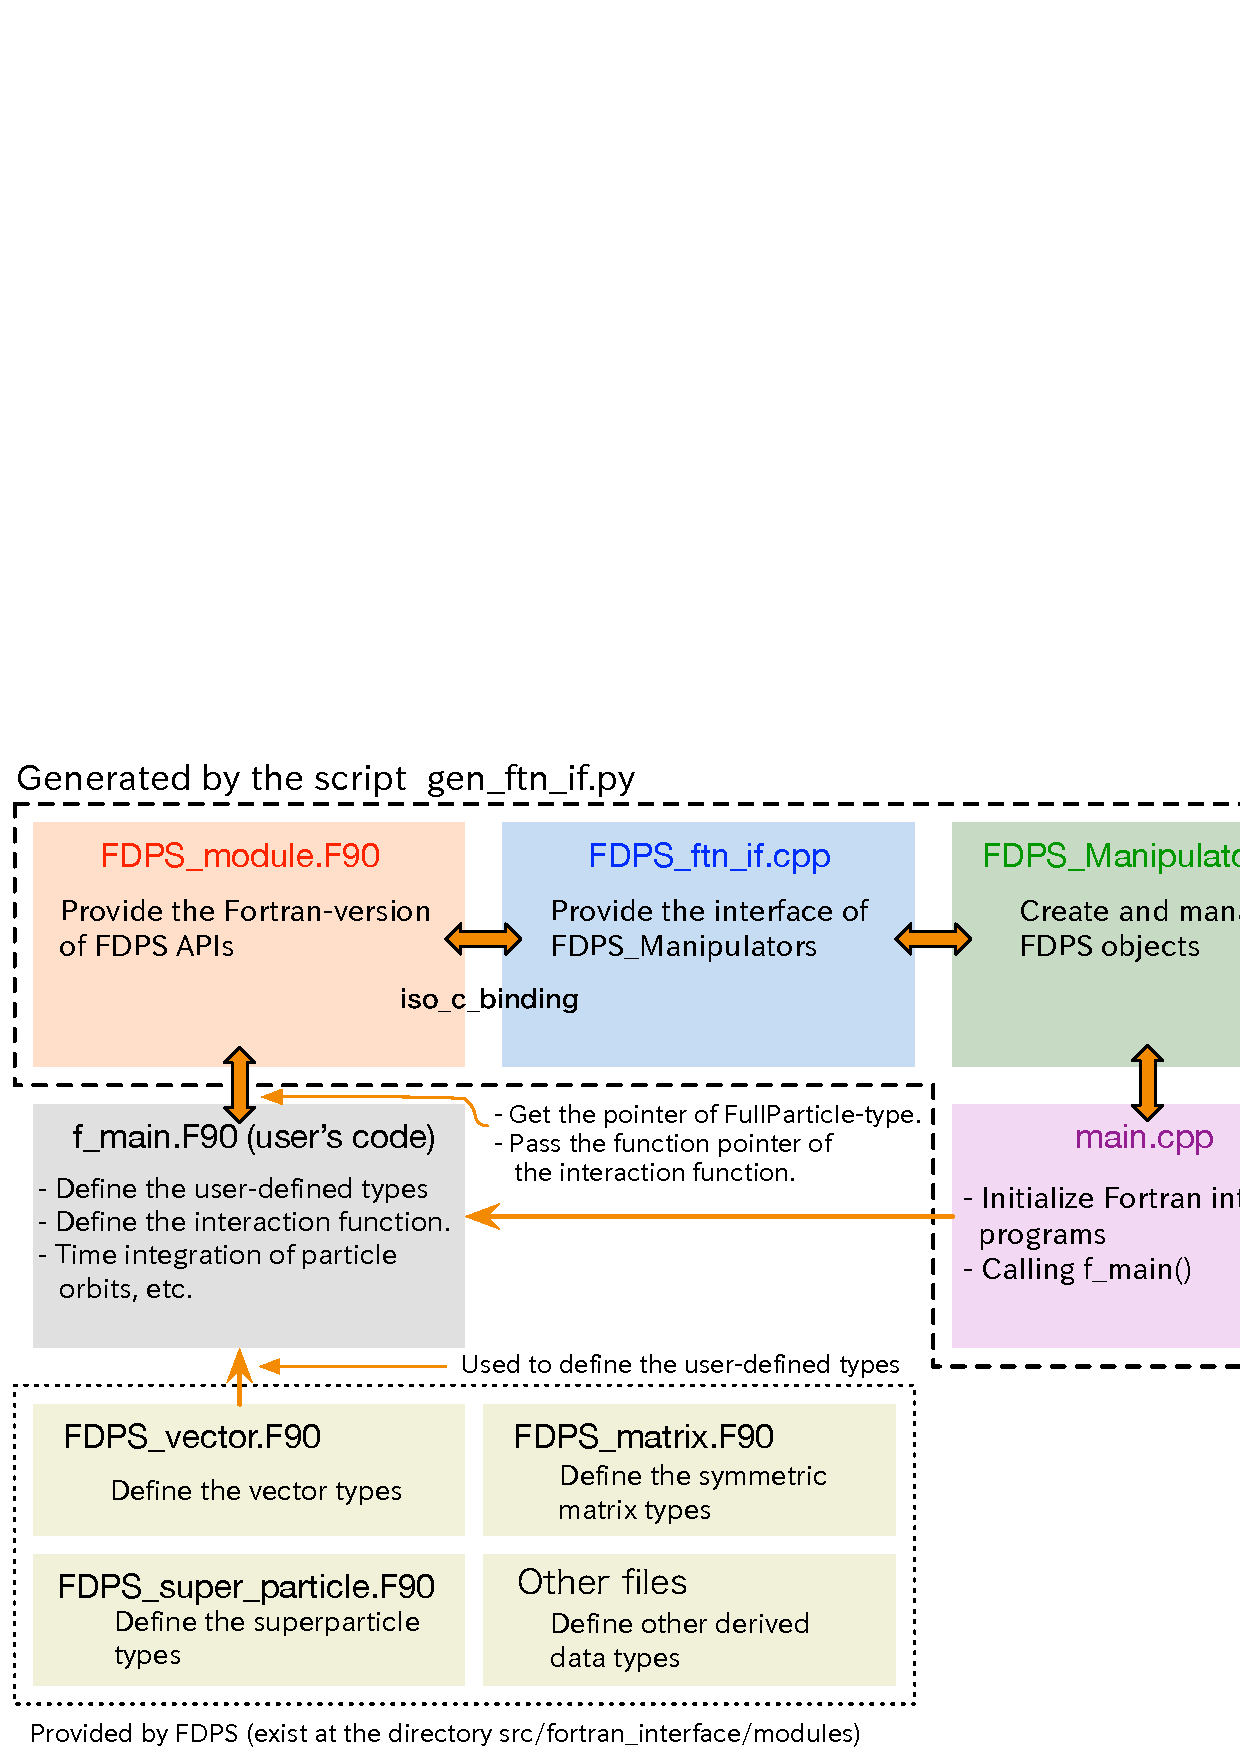
\includegraphics[width=\linewidth]{./fig/FDPS_ftn_if_file_str.pdf}
\caption{Fortran インターフェースとユーザコードの関係。}
\label{fig:FDPS_ftn_if_file_str}
\end{figure}


まず\path{FDPS_Manipulators.cpp}と\path{main.cpp}について説明する。FDPS 本体はC++で記述されているため、第\ref{chap:overview}章「FDPS 概要」で説明した領域クラス、粒子群クラス、相互作用ツリークラスのC++オブジェクトは、すべてC++ファイル内で生成し、管理する必要がある。これを行うのが、\path{FDPS_Manipulators.cpp}である。同様の理由によって、実行プログラムの\path{main}関数はC++ファイルに置く必要がある。そのため、\path{main.cpp}が生成される。この\path{main.cpp}では\path{f_main()}という名称のFortranのサブルーチンを呼び出す。したがって、ユーザはFortran サブルーチン \path{f_main()}を用意し、その中にユーザコードを実装する必要がある。詳細は第\ref{chap:API_spec_list}章「API 仕様一覧」に譲るが、\path{FDPS_Manipulators.cpp}で生成されるC++オブジェクトは、Fortranの整数変数に割り当てられる。したがって、ユーザはこれらのオブジェクトを整数変数を使って管理することとなる。

次に\path{FDPS_ftn_if.cpp}について説明する。FortranはC++の関数を直接呼び出して使用することはできないが、Fortran 2003の機能(Fortranモジュール\path{iso_c_binding}で提供される機能のこと)を使用することで、C言語の関数を呼び出すことが可能になる。そこで、本 FDPS Fortran インターフェースでは、\path{FDPS_Manipulators.cpp}内で定義される各種のC++関数のC言語インターフェースを別途用意し、これらをFortranから呼び出して、FDPSを操作する仕組みとした。これらC言語インターフェースが\path{FDPS_ftn_if.cpp}に実装されている。

最後に、\path{FDPS_module.F90}について説明する。\path{FDPS_module.F90}は、C言語インターフェースを呼び出すための派生データ型\path{FDPS_controller}をユーザに提供する。この\path{FDPS_controller}は、Fortran 2003のクラス(メンバ関数を持つ派生データ型のこと)であり、そのメンバ関数がFDPSのFortran用インターフェースを与える。メンバ関数、すなわち、Fortran インターフェースの一覧は第\ref{chap:API_spec_list}章「API 仕様一覧」で記述する。\path{FDPS_controller}は、\path{FDPS_module.F90}において、以下のように定義されている(リスト\ref{listing:FDPS_module_str}):
\begin{lstlisting}[caption=\texttt{FDPS\_module.F90}の構造,label=listing:FDPS_module_str]
module FDPS_module
   use, intrinsic :: iso_c_binding
   implicit none
   
   !**** FDPS controller
   type, public :: FDPS_controller
   contains
      !
      ! APIs are defined here.
      !
   end type FDPS_controller
   
end module FDPS_module  
\end{lstlisting}
見やすさのため、上記のリストにおいて、メンバ関数の宣言部の記述は省略している。実際には、各メンバ関数の宣言が、文字列\verb|contains|と文字列\verb|end type FDPS_controller|の間の領域に記述される。このような仕様のため、ユーザはユーザコードにおいて、以下の手順でFortranインターフェースを使用する必要がある:
\begin{enumerate}[leftmargin=*,itemsep=-1ex,label=(\arabic*)]
\item モジュール\path{FDPS_module}を\path{use}する
\item クラス\path{FDPS_controller}のオブジェクトを生成する
\item 生成した\path{FDPS_controller}オブジェクトのメンバ関数を呼び出す
\end{enumerate}
最も単純な使用例をリスト\ref{listing:simple_example_ftn_if}に示す:
\begin{lstlisting}[caption=Fortranインターフェースの使用例,label=listing:simple_example_ftn_if]
subroutine f_main()
   use FDPS_module ! Step (1)
   implicit none
   type(FDPS_controller) :: fdps_ctrl ! Step (2)
   
   ! Call Fortran interface
   call fdps_ctrl%PS_initialize() ! Step (3)
   
end subroutine f_main
\end{lstlisting}
リスト中にコメントで示された番号は、上の手順の番号に対応している。

%%%%%%%%%%%%%%%%%%%%%%%%%
\subsection{C言語 インターフェース}
\label{subsec:file_str_c_if}
C言語の場合もFortranの場合と全く同様に、C言語 インターフェースプログラムを通して、FDPSの機能を使用することになる。C言語 インターフェースプログラムの生成は、ユーザがディレクトリ\path{scripts}の下に置かれたスクリプト\path{gen_c_if.py}を実行することで行われる。このスクリプトは、FDPSを利用するにあたってユーザ自身が定義(実装)しなければならない構造体(同様に\textbf{ユーザ定義型}と呼称)を解析して、インターフェースプログラムを生成する。C言語でユーザ定義型を実装するのに必要となるC言語ヘッダーファイルが\path{src/c_interface/headers}に、インターフェース生成時に設計図として使用されるファイル群が \path{src/c_interface/blueprints} に配置されている。

図\ref{fig:FDPS_c_if_file_str}に、C言語用インターフェースプログラムの生成が正常に行われた場合の C言語 インターフェースのファイル構成とその役割を示している。図の破線で囲まれた4つのファイル(\path{FDPS_c_if.h}, \path{FDPS_ftn_if.cpp}, \path{FDPS_Manipulators.cpp}, \path{main.cpp})がスクリプトによって生成されるC言語インターフェースプログラムであり、\path{c_main.c}がユーザ側が用意するプログラムである。図の点線で囲まれたファイル(\path{FDPS_basic.h}、\path{FDPS_enum.h}、\path{FDPS_vector.h}、\path{FDPS_matrix.h}、\path{FDPS_super_particle.h}等)は、前述したように、ユーザがユーザ定義型およびユーザ定義関数(第\ref{chap:overview}章参照)を記述するのに必要な構造体の定義を与えるものである。図からわかるように、ファイル構成は、Fortranインターフェースプログラムと非常に類似した構成となっており(図\ref{fig:FDPS_ftn_if_file_str}参照)、特に同名のファイルの役割はFortranインターフェースで説明したファイルと全く同じである。以下、異なる部分についての注意書きのみを記す。


%%% 図:全体のファイル構成
\begin{figure}[h]
\centering
\includegraphics[width=\linewidth]{./fig/FDPS_c_if_file_str.pdf}
\caption{C言語 インターフェースとユーザコードの関係。}
\label{fig:FDPS_c_if_file_str}
\end{figure}

\begin{itemize}[leftmargin=*]
\item 実行ファイルの\path{main}関数は\path{main.cpp}にある。この\path{main.cpp}では\path{c_main()}という名称の\texttt{void}関数を呼び出す。したがって、ユーザは\texttt{void}関数 \path{c_main()}を用意し、その中にユーザコードを実装する必要がある。
\item FDPSのC言語用APIのプロトタイプ宣言は\path{FDPS_c_if.h}に記述されている。したがって、ユーザはFDPSの機能を利用するため、このファイルをインクルードする必要がある。\path{FDPS_c_if.h}では、FDPSが提供する構造体の定義が記述されたヘッダーファイル群(\path{FDPS_basic.h}等)がインクルードされているため、ユーザはこのファイルのみをインクルードすれば、これら構造体をユーザコードの中で利用することができる。
\end{itemize}


%%%%%%%%%%%%%%%%%%%%%%%%%
\subsection{Fortran/C言語 インターフェースを使ったコード開発の流れ}
本節では、FDPSのFortran/C言語 インターフェースを使ったユーザコード開発の流れについて記述する。大まかな流れは以下のようになる:
\begin{enumerate}[leftmargin=*,label={[\arabic*]}]
\litem{ユーザ定義型の実装} 前節で述べた通り、FDPSのFortran/C言語 インターフェースを生成するためには、はじめにユーザ定義型を実装しなければならない。ユーザ定義型はFortranでFDPSを利用する場合には派生データ型で、C言語でFDPSを利用する場合には構造体として実装する。ユーザ定義型の記述方法の詳細は、第\ref{chap:user_defined}章で説明する。
\litem{インターフェースプログラムの生成} ユーザ定義型の実装が完了したら、インターフェース生成用スクリプト \path{gen_ftn_if.py} または \path{gen_c_if.py} を使って、インターフェースプログラムを生成する。生成が完了した時点で、ユーザはFDPSのFortran/C言語用インターフェースをユーザコードの中で使用することができるようになる。スクリプトの使用法と仕様については第\ref{chap:script_spec}章で説明する。
\litem{ユーザ定義関数の実装} ユーザは相互作用を記述する関数(ユーザ定義関数)を実装しなければならない。ユーザ定義関数は、Fortranではサブルーチン、C言語では\texttt{void}関数として実装する。ユーザ定義関数の記述方法の詳細は、第\ref{chap:user_defined}章で説明する。
\litem{ユーザコードの開発} ユーザ定義型、ユーザ定義関数、FDPS APIを用いて、ユーザが行いたい粒子シミュレーションコードを開発する。この際、次の点に注意して開発を行う必要がある:
\begin{itemize}
\item ユーザコードはFortranのサブルーチン\path{f_main()}、或いは、C言語の\texttt{void}関数 \path{c_main()}の中に実装しなければならない。
\item FDPS Fortran インターフェースのAPIは、クラス\path{FDPS_controller}のメンバ関数として提供される。したがって、FDPS APIはメンバ関数を呼び出して使用する。一方、FDPS C言語 インターフェースのAPIのプロトタイプ宣言は、\path{FDPS_c_if.h}でなされているため、このファイルをインクルードすることでAPIを呼び出すことが可能となる。
\end{itemize}
Fortran インターフェースを用いたコードの例に関しては、\path{sample/fortran}の下で提供されているサンプルコードを参照して頂きたい(第\ref{sec:sample_codes}節も参照のこと)。一方、C言語 インターフェースを用いたサンプルコードは、\path{sample/c}の下に用意されている。
\litem{コンパイル} ユーザコードの実装が完了したら、コンパイルを行い、実行プログラムを得る。前節で述べたように、インターフェースプログラムはC++言語と、Fortran言語或いはC言語のソースファイルが混在した構成となっており、単一の言語のみで構成されたプログラムとは異なる仕方でコンパイルする必要がある。この点に関しての詳細は、第\ref{chap:compile_and_macro}章で解説する。FDPSではコンパイル時のマクロ定義を使い、いくつかの設定を行うことが可能である。これに関しても、第\ref{chap:compile_and_macro}章で解説する。拡張機能 Particle Mesh を使用する場合には、事前に必要なライブラリをインストールし、コンパイル時に適切にライブラリを指定することが必要である。
\litem{実行} コンパイルして得られる実行ファイルは、通常の実行ファイルと違いはない。ユーザが利用している計算機環境の利用規則に則って、実行ファイルを実行する。
\end{enumerate}

%%%%%%%%%%%%%%%%%%%%%%%%%
\subsection{インターフェースプログラム生成の必要性}
\label{subsec:reasons_for_autogen_ftn_if}
前々節で述べたように、FDPSのFortran/C言語用インターフェースはライブラリの形で提供されるものではなく、インターフェースプログラムのソースコードの形で提供される。本節では、この理由について解説を行う。

まず、準備として、C++でのFDPSの使用について概説する。第\ref{chap:overview}章\ref{subsec:things_to_do_by_users}節で述べた通り、FDPSではユーザは粒子や相互作用の定義を自由に行うことができ、これによって、FDPSは様々なタイプの粒子シミュレーションに対して適用可能となっている。この自由度を実現するため、FDPS 本体の関数はC++のテンプレート機能を用いて記述されている。ここで、テンプレート機能とは、Fortranでいうサブルーチンや関数(或いはC言語の関数)に、(変数ではなく)データ型を引数として受け取れるようにする機能のことである。この機能によって、C++では仮のデータ型を使用して関数を記述することが可能となる(この仮のデータ型はコンパイル時に具体的なデータ型になってさえいればよい)。また、FDPS 本体はC++のヘッダファイルの形で提供される。したがって、C++でFDPSを使用する場合、ユーザはFDPSのヘッダファイルをユーザコードの中でインクルードし、FDPS APIのテンプレート引数にユーザが定義した粒子型を指定して使用する。ユーザコードのコンパイル時には、FDPS APIの関数で使用されるすべての変数のデータ型が決定されているため、コンパイラは問題なくユーザプログラムをコンパイルすることが可能となっているのである。

FortranやC言語にはテンプレート機能に相当するものは存在しないため、仮の(或いは、未定の)データ型を用いてサブルーチンや関数を実装する、ということはFortranやC言語では不可能である。これが、Fortran/C言語用インターフェースをライブラリの形で提供できない1つの理由である。我々は、FortranやC言語においてもユーザが粒子や相互作用の定義を自由に行えるようにするため、ユーザが実装した粒子の派生データ型/構造体等を調べ、それに応じて適切なAPIを自動的に生成する方法を採用している。

もう1つの理由は、C++で実装されたFDPSをそのまま使用しているからである。C++で記述されたFDPSとFortran 或いは C言語のプログラムの間でデータをやり取りするためには、FortranやC言語で記述された粒子型と同等な粒子クラスをC++側に用意する必要がある。これにもユーザが実装した派生データ型や構造体を解析して生成するという作業が必要となる。

以上の理由により、FDPS Fortran/C言語 インターフェースは、ソースコードで提供される形となっている。

%%%%%%%%%%%%%%%%%%%%%%%%%%%%%%%%%%%%%%%%%%%%%%%%%%%%
\section{ドキュメント}
ドキュメント関係のファイルはディレクトリ \path{doc} の下にある。サンプルコードを使ってFDPS Fortran インターフェースの基本的な使用法を解説するチュートリアル文書が \path{doc_tutorial_ftn_ja.pdf} である。C言語 インターフェースの基本的な使用方法についてのチュートリアル文書は\path{doc_tutorial_c_ja.pdf}である。仕様書(本文書)が \path{doc_specs_ftn_ja.pdf} である。

%%%%%%%%%%%%%%%%%%%%%%%%%%%%%%%%%%%%%%%%%%%%%%%%%%%%
\section{サンプルコード}
\label{sec:sample_codes}
FortranとC言語のサンプルコードが、それぞれ、ディレクトリ \path{sample/fortran} 及び \path{sample/c} の下にある。サンプルコードは4つ用意されており、それぞれ、無衝突系の重力 $N$ 体シミュレーションコード(\path{sample/fortran/nbody}, \path{sample/c/nbody})、固定長カーネルを使った SPH シミュレーションコード(\path{sample/fortran/sph}, \path{sample/c/sph})、$\mathrm{P^{3}M}$(Particle-Particle-Particle-Mesh) 計算用コード(\path{sample/fortran/p3m}, \path{sample/c/p3m})、円盤銀河の$N$体/SPHシミュレーションコード(\path{sample/fortran/nbody+sph}, \path{sample/c/nbody+sph})となっている。
